\chapter{Diseño y desarrollo de la aplicación\label{sec:disenho}}

TODO: Diseño del proyecto

\lsection{Arquitecturas de captura}


%Arquitectura de captura tradicional

\begin{figure}[!th]
\centering
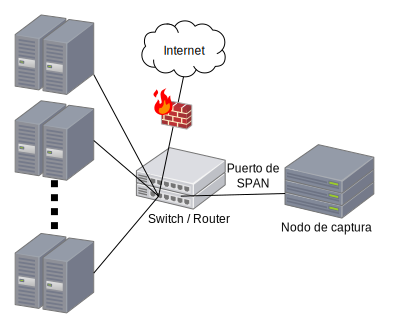
\includegraphics[scale=.7]{arq}
\caption{Arquitectura de captura tradicional}
\label{fig:dis:arq}
\end{figure}

%Arquitectura en un sistema virtual

\begin{figure}[!th]
\centering
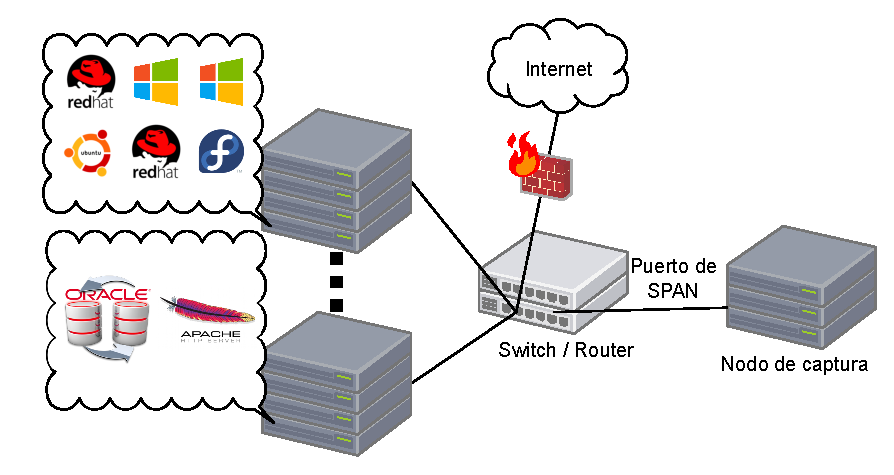
\includegraphics[scale=.7]{arqvm}
\caption{Arquitectura de captura en un sistema con virtualización}
\label{fig:dis:arqvm}
\end{figure}

%Arquitectura en un sistema completo virtual

\begin{figure}[!th]
\centering
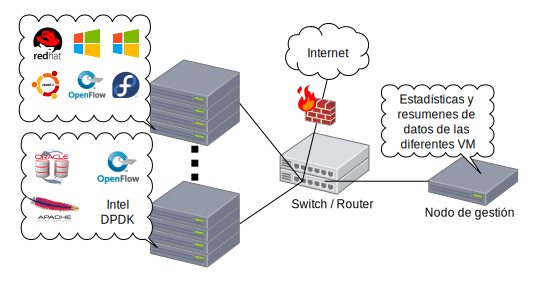
\includegraphics[scale=.7]{arqfullvm}
\caption{Arquitectura de un sistema de captura completamente virtualizado}
\label{fig:dis:arqfullvm}
\end{figure}

\lsection{Sistema de captura diseñado}


\begin{figure}[!th]
\centering
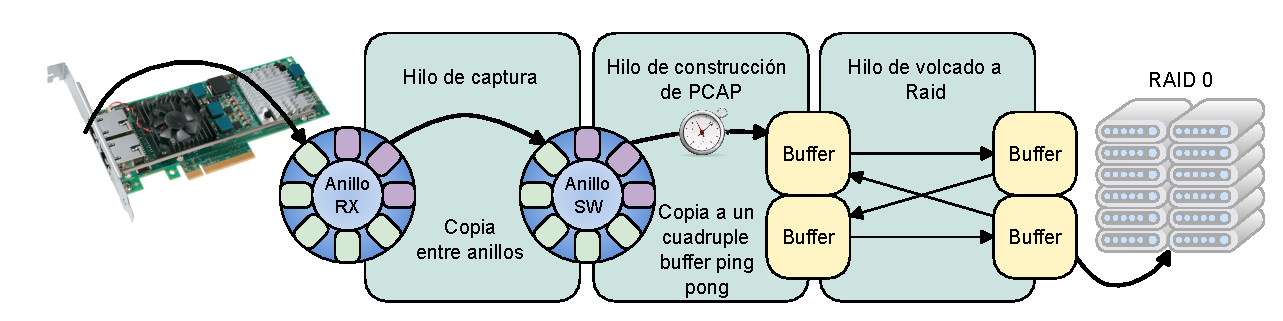
\includegraphics[scale=.7]{dpdkdd}
\caption{Arquitectura de un sistema de captura con DPDK}
\label{fig:dis:dpdkdd}
\end{figure}


